\hsection{\crowsFoot{A}{O1}{B}{O1}}%
\label{sec:rm:ab}%
%
\begin{figure}%
\centering%
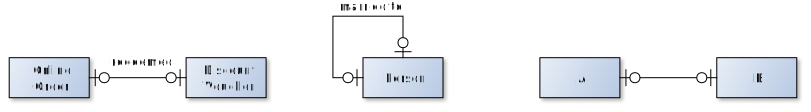
\includegraphics[width=0.97\linewidth]{\currentDir/AB}%
\caption{Examples of the \crowsFoot{A}{O1}{B}{O1} relationship pattern from back in \dref{sec:conceptual:relationshipCardinalities}.}%
\label{fig:rm:ab}%
\end{figure}%
%
\gitLoadAndExecSQL{AB_1_tables}{}{conceptualToRelational}{AB_1_tables.sql}{relationships}{}{}%
\listingSQLandOutput{AB_1_tables}{%
The three-table realization of an \crowsFoot{A}{O1}{B}{O1} conceptual relationship.%
}{}%
\gitLoadAndExecSQL{AB_1_insert_and_select}{}{conceptualToRelational}{AB_1_insert_and_select.sql}{relationships}{}{}%
\listingSQLandOutput{AB_1_insert_and_select}{%
Inserting into and selecting data from the three-table realization of an \crowsFoot{A}{O1}{B}{O1} conceptual relationship given in \cref{lst:AB_1_tables}.%
}{}%
%
\gitExec{cdtrmTableAO}{\databasesCodeRepo}{conceptualToRelational}{../_scripts_/db_table_to_latex_table.sh relationships a aid;x}%
\gitExec{cdtrmTableBO}{\databasesCodeRepo}{conceptualToRelational}{../_scripts_/db_table_to_latex_table.sh relationships b bid;y}%
\gitExec{cdtrmTableRAB}{\databasesCodeRepo}{conceptualToRelational}{../_scripts_/db_table_to_latex_table.sh relationships relate_a_and_b fkaid;fkbid}%
%
\begin{figure}%
\centering%
\floatSep%
\centering\input{\gitFile{cdtrmTableAO}}%
\floatSep%
\centering\input{\gitFile{cdtrmTableBO}}%
\floatSep%
\centering\input{\gitFile{cdtrmTableRAB}}%
\floatSep%
\caption{The contents of the the tables in the three-table implementation of the \crowsFoot{A}{O1}{B}{O1} conceptual relationship after executing \cref{lst:AB_1_insert_and_select}.}%
\label{fig:rm:ab:1:tables}%
\end{figure}%
%
\gitLoadAndExecSQL{AB_1_insert_error_1}{}{conceptualToRelational}{AB_1_insert_error_1.sql}{relationships}{}{}%
\listingSQLandOutput{AB_1_insert_error_1}{%
The schema illustrated in \cref{lst:AB_1_tables} prevents entities of type~A to be related to more than one entity of type~B.%
}{}%
\gitLoadAndExecSQL{AB_1_insert_error_2}{}{conceptualToRelational}{AB_1_insert_error_2.sql}{relationships}{}{}%
\listingSQLandOutput{AB_1_insert_error_2}{%
The schema illustrated in \cref{lst:AB_1_tables} prevents entities of type~B to be related to more than one entity of type~A.%
}{}%
\gitLoadAndExecSQL{AB_cleanup}{}{conceptualToRelational}{AB_cleanup.sql}{relationships}{}{}%
\listingSQLandOutput{AB_cleanup}{%
Deleting the three tables again, because we want to try another realization of the \crowsFoot{A}{O1}{B}{O1} conceptual relationship.%
}{}%
%
\gitLoadAndExecSQL{AB_2_tables}{}{conceptualToRelational}{AB_2_tables.sql}{relationships}{}{}%
\listingSQLandOutput{AB_2_tables}{%
The two-table realization of an \crowsFoot{A}{O1}{B}{O1} conceptual relationship.%
}{}%
\gitLoadAndExecSQL{AB_2_insert_and_select}{}{conceptualToRelational}{AB_2_insert_and_select.sql}{relationships}{}{}%
\listingSQLandOutput{AB_2_insert_and_select}{%
Inserting into and selecting data from the two-table realization of an \crowsFoot{A}{O1}{B}{O1} conceptual relationship given in \cref{lst:AB_2_tables}.%
}{}%
%
\gitExec{cdtrmTableAT}{\databasesCodeRepo}{conceptualToRelational}{../_scripts_/db_table_to_latex_table.sh relationships a aid;fkbid;x}%
\gitExec{cdtrmTableBT}{\databasesCodeRepo}{conceptualToRelational}{../_scripts_/db_table_to_latex_table.sh relationships b bid;y}%
%
\begin{figure}%
\centering%
\floatSep%
\input{\gitFile{cdtrmTableAT}}%
\floatSep%
\input{\gitFile{cdtrmTableBT}}%
\floatSep%
\caption{The contents of the the tables in the two-table implementation of the \crowsFoot{A}{O1}{B}{O1} conceptual relationship after executing \cref{lst:AB_2_insert_and_select}.}%
\label{fig:rm:ab:2:tables}%
\end{figure}%
%
\gitLoadAndExecSQL{AB_2_insert_error_2}{}{conceptualToRelational}{AB_2_insert_error_2.sql}{relationships}{}{}%
\listingSQLandOutput{AB_2_insert_error_2}{%
The schema illustrated in \cref{lst:AB_2_tables} prevents entities of type~B to be related to more than one entity of type~A via constraints. %
The entities of type~A can only be associated with one entity of type~B because of the table structure.%
}{}%
%
We have the two entity types~A and~B.
Each entity of type~A is connected to zero or one entity of type~B.
Each entity of type~B is connected to zero or one entity of type~A.

We saw examples of this relationship pattern back in \dref{sec:conceptual:relationshipCardinalities}:
Let's we are a pizzeria that allows customers to order pizzas online.
We also hand out discount vouchers that allow can reduce the cost of an online order by~20\%.
Each voucher can be redeemed for one such online order or it may also not be redeemed at all.
For each online order, you may use one voucher to reduce the cost, or you may not use any voucher at all.

Another example could be integrated into our teaching management platform.
As you will remember, we used the entity type~\emph{Person} as central model component.
If we wanted, we could add information about the current marital status of all people in form of, fittingly, relationships.
Each person can be married to zero or one (other) person.
These two examples are illustrated in \cref{fig:rm:ab}.

There are two possible ways to implement this relationship pattern in a relational \dbms:%
%
\begin{enumerate}%
%
\item We can use a three-table solution, where each entity type gets one table and the relationship between the entity types~A and~B is managed in a third table.
This solution makes sense if we have only few pairs of~A and B~entities that are related.%
%
\item We can use a two-table solution, where we manage the relationship with an additional column in one of the tables.
This is the better solution if we have many related pairs of~A and B~entities.%
%
\end{enumerate}%
%
Regardless which solution we pick, we need at least the following two tables.
First, table~\sqlil{a} is used for the entity type~A.
As primary key, we here use a surrogate primary key~\sqlil{aid} which is an automatically generated integer sequence.
Let us assume that the entity type~A also has a feature~\sqlil{x}, for illustration purposes, a string composed of three characters.
Second, table~\sqlil{b} for the entity type~B.
We here use a surrogate primary key~\sqlil{bid}, again an automatically generated integer sequence.
Assume that there also is an attribute~\sqlil{y}, which is a string of two characters.
(In all the remaining examples in this section, we will use similar table patterns).

We start with the three-table approach in~\cref{lst:AB_1_tables}, as suggested in, e.g.,~\cite{S2024D:MEDTRDM}.
There, we have a third table~\sqlil{relate_a_and_b} relating the entities of type~A to those of type~B.
This table has two columns, the first one, \sqlil{fkaid}, holding the primary key of the A~entities as foreign key and the second one, \sqlil{fkbid}, holding the primary key of the B~entities as foreign key.
Since we only store the pairs that exist, both columns have the~\sqlil{NOT NULL} constraint.
Both also have~\sqlil{REFERENCES} constraints to their respective foreign keys.
Since on both relationship ends there can only be one entity, both columns also have \sqlil{UNIQUE}~constraints.
Either of them may be used as~\sqlil{PRIMARY KEY}.

We would probably choose the key belonging from the most common direction in which we access the table.
If we most likely look for fitting entities of type~B coming from a row representing an entity of type~A~(as is the case in \cref{lst:AB_1_insert_and_select}), then we would probably use~\sqlil{fkaid} as \sqlil{PRIMARY KEY}.
If it was the other way around, we would pick~\sqlil{fkbid}.

In \cref{lst:AB_1_insert_and_select}, we fill some data into the tables.
Since both relationship ends are optional, we can begin by inserting data into tables~\sqlil{a} and~\sqlil{b} without specifying any references to the other table.
We do not need to specify the primary keys, since the are automatically generated, and, as said, we can omit the foreign keys, because they are allowed to be~\sqlil{NULL}.
So we only need to provide values for the attributes~\sqlil{x} and~\sqlil{y}.
After this, we have filled both tables with some data.
We can then establish relationships between the rows of tables~\sqlil{a} and~\sqlil{b} by adding entries to~\sqlil{relate_a_and_b} with the primary keys of the related rows.
\sqlil{INSERT INTO relate_a_and_b (fkaid, fkbid) VALUES (2, 3);}, for example, would relate the row in table~\sqlil{a} with~\sqlil{aid = 2} to the row in table~\sqlil{b} with~\sqlil{bid = 3}.
The contents of the tables after executing \cref{lst:AB_1_insert_and_select} is illustrated in \cref{fig:rm:ab:1:tables}.

Now we want to query some information about~A, using~\sqlil{SELECT}, but also need information about the potentially related~B.
We use an~\sqlil{INNER JOIN} coming from table~\sqlil{a} on the third table~\sqlil{relate_a_and_b} based on the primary key~\sqlil{aid} of table~\sqlil{a}.
We then need another~\sqlil{INNER JOIN} with the table for~B on its primary key~\sqlil{bid}, as shown in \cref{lst:AB_1_insert_and_select}.
This way, we can reconstruct the related data in two steps.

Notice that it is impossible to have any row of table~\sqlil{a} that is related to more than one row in table~\sqlil{b}, as demonstrated in \cref{lst:AB_1_insert_error_1}.
The \sqlil{UNIQUE} constraint on the column~\sqlil{a} of~\sqlil{relate_a_and_b} prevents this.
Vice versa, the \sqlil{UNIQUE} constraint on column~\sqlil{b} in~\sqlil{relate_a_and_b} prevents that any row in table~\sqlil{b} is related to more than one row in table~\sqlil{a}.
This is demonstrated in \cref{lst:AB_1_insert_error_2}.

However, there are two problems with this three-table-method:
First, we need two \sqlil{INNER JOIN} statements to combine the data from the entities~A and~B.
Second, this approach makes sense only if comparatively \emph{few}~pairs of related A~and B~entities exist.
Performance and space-wise, in the worst case, all entities of type~A are related to an entity of type~B or vice versa.
In other words, our third table can be about as big as the smaller one of the two other tables.
If the tables are big, then the query may not be fast.
Also, if all entities of type~A were related to an entity of type~B, then we could just as well reference these B~entities directly from the table for entity type~A.
Actually, in that case, using the third table would just be a waste of space and query time.

Thus, if many or most A~entities are related to B~entities, then instead of using a third table, we could alternatively add a column~\sqlil{fkbid} to the table for~A and store the primary keys of the related B~entities in that column.
We delete the tables we just created in \cref{lst:AB_cleanup} to explore the two-table solution in \cref{lst:AB_1_tables}.
The new column~\sqlil{fkbid} added to the table~\sqlil{a} can be allowed to be~\sqlil{NULL}, because not all entities of type~A need to be related to an entity of type~B.
It must be marked as \sqlilIdx{UNIQUE}, though, because no entity of type~B can be related to more than one entity of type~A.
This constraint only applies to values that are \emph{not}~\sqlil{NULL}.

It also needs a \sqlil{REFERENCES} constraint.
In \cref{lst:AB_2_tables}, we add this constraint later via \sqlil{ALTER TABLE}\sqlIdx{ALTER!TABLE}\sqlIdx{TABLE}, very much like \pgmodeler\ does it~(see back in \cref{lst:logical:teachingManagment:student_database_2:05_public_mobile_mobile_student_id_fk_constraint_5087}).
Otherwise, we would need to create table~\sqlil{b} before table~\sqlil{a}.
That is totally OK, but if we had many tables, the required order of table creation could make our \sql\ code harder to read.
Also, the probability of making errors that are hard to figure out would be higher.
It sometimes is just easier to first create the tables and then add the constraints via \sqlIdx{ALTER TABLE}.
I guess this is why \pgmodeler\ does it like this, too.

We could also do this vice versa, i.e., add an column~\sqlil{fkaid} to table~\sqlil{b} instead.
Either way, this removes the need for a third table.

In \cref{lst:AB_2_insert_and_select}, we insert the data into the two tables~\sqlil{a} and~\sqlil{b} exactly as before.
The relationships are now no longer inserted into a third table.
Instead, we use \sqlilIdx{UPDATE} statements~\cite{PGDG:PD:U}, as illustrated in \cref{lst:AB_2_insert_and_select}.
\sqlil{UPDATE a SET fkbid = 3 WHERE aid = 2;}, for example, relates the row in table~\sqlil{a} with~\sqlil{aid = 2} to the row in table~\sqlil{b} with~\sqlil{bid = 3}.
The contents of the tables after creating the data is illustrated in~\cref{fig:rm:ab:2:tables}.
We can now recombine the data from the two tables using a single~\sqlil{INNER JOIN}.

Relating entities of type~A to multiple entities of type~B is impossible, because the column~\sqlil{fkbid} in table~\sqlil{a} can only have one value.
Relating entities of type~B to multiple entities of type~A is impossible, because of the \sqlil{UNIQUE} constraint imposed on it the column~\sqlil{fkbid} in table~\sqlil{a}.
A failed attempt to do so anyway is shown in \cref{lst:AB_2_insert_error_2}.

Of course, the table for entity type~A now needs more space.
If only few entities of type~A are related to entities of type~B, maybe the first solution, based on three tables, is maybe better.
I think most often, the second solution, the two-table approach, is the way to go.
Still, it depends on how many of the A~and B~entities are related, from which \inQuotes{side} we most likely navigate the relationship, and how big the tables are.%
%
\FloatBarrier%
\endhsection%
